\documentclass[11pt,letterpaper]{article}

\usepackage[letterpaper,margin=0.8in,nohead]{geometry}

\usepackage[colorlinks]{hyperref}
\usepackage{url}
\usepackage{breakurl}

\hypersetup{
	colorlinks,
	linkcolor={red},
	citecolor={red},
	urlcolor={blue}
}

\usepackage{verbatim}
\usepackage{fancyvrb}
\usepackage{scrextend}
\usepackage{enumitem}
\usepackage{url}
\usepackage{tabularx}

\usepackage{caption}
\usepackage{graphicx}
\usepackage{float}
\usepackage{subcaption}

\usepackage{changepage}   % for the adjustwidth environment

\newenvironment{answer}{\em \color{blue} \begin{adjustwidth}{1cm}{1cm}}{\end{adjustwidth}}

% math
\usepackage{amsthm,amsmath}
\usepackage{amsfonts}

\newcommand{\mc}[1]{\mathcal{#1}}	% Mechanisms / Algorithms
\newcommand{\rv}[1]{\mathbf{#1}}    % Random variable

\newcommand{\pr}[1]{\mathrm{Pr}\{#1\}} % Probability

\newtheorem{corollary}{\bf Corollary}%[theorem]
\newtheorem{lemma}{\bf Lemma}%[theorem]
\newtheorem{definition}{\bf Definition}%[section]

\newtheorem{observation}{\bf Observation}%[theorem]

% load cleveref last!
\usepackage[capitalise]{cleveref}


\begin{document}
	
	\title{EN4720: Security in Cyber-Physical Systems \\ Exercise --- Encryption and Hashing}
	
	%% This is an individual assignment!!
	%% TODO: put your name and index number here here!
	\author{ \textcolor{blue}{Name: Thalagala B. P.} \\ \textcolor{blue}{Index No: 180631J}}
	
	\maketitle
	
	\begin{center}
		\color{red}\bf This is an individual exercise! \\ Due Date: 21 April 2022 by 11.59 PM
	\end{center}
	
	% \subsection*{Problem 1 - Block Cipher Modes of Operation}
	
	% Critically analyze block ciper modes of operation and fill the following table. You may search on the internet/refer to existing literature and discuss among friends to answer this question.  But plagiarism will not be tolerated! Make sure you add the relevant citations. One citation is given to you as an example below.
	% \vspace{2mm}
	
	% \noindent ``Recommendation for block cipher modes of operation'' published by NIST is a good resource to get started with~\cite{dworkin2001recommendation}.
	
	% \begin{table}[htbp]
		%     \caption{Comparison of modes of operation
			%     }
		%     \begin{tabularx}{\columnwidth}{|p{2cm}|X|X|X|}
			%         \hline
			%         \textbf{Mode} & \textbf{Pros}       & \textbf{Cons} & \textbf{Usage examples}  \\
			%         \hline
			%         ECB & 
			%         Pro 1 | Pro 2 | Pro 3 & 
			%         Con 1 | Con 2 | Con 3 & 
			%         Example 1 | Example 2 | Example 3 \\ \hline
			
			%         \hline
			%         CBC & 
			%         Pro 1 | Pro 2 | Pro 3 & 
			%         Con 1 | Con 2 | Con 3 & 
			%         Example 1 | Example 2 | Example 3 \\ \hline
			
			%         \hline
			%         CFB & 
			%         Pro 1 | Pro 2 | Pro 3 & 
			%         Con 1 | Con 2 | Con 3 & 
			%         Example 1 | Example 2 | Example 3 \\ \hline
			
			%         \hline
			%         OFB & 
			%         Pro 1 | Pro 2 | Pro 3 & 
			%         Con 1 | Con 2 | Con 3 & 
			%         Example 1 | Example 2 | Example 3 \\ \hline
			
			%         \hline
			%         CTR & 
			%         Pro 1 | Pro 2 | Pro 3 & 
			%         Con 1 | Con 2 | Con 3 & 
			%         Example 1 | Example 2 | Example 3 \\ \hline
			%     \end{tabularx}
		% \end{table}
	
	\subsection*{Problem 1 - Symmetric Encryption \& Key Exchange}
	
	Alice and Bob are using the Diffie-Hellman protocol as shown in Figure~\ref{fig:dh-protocol}. They want to extend their key exchange mechanism to include their friend Charlie.
	
	\begin{figure}[h]
		\centering
		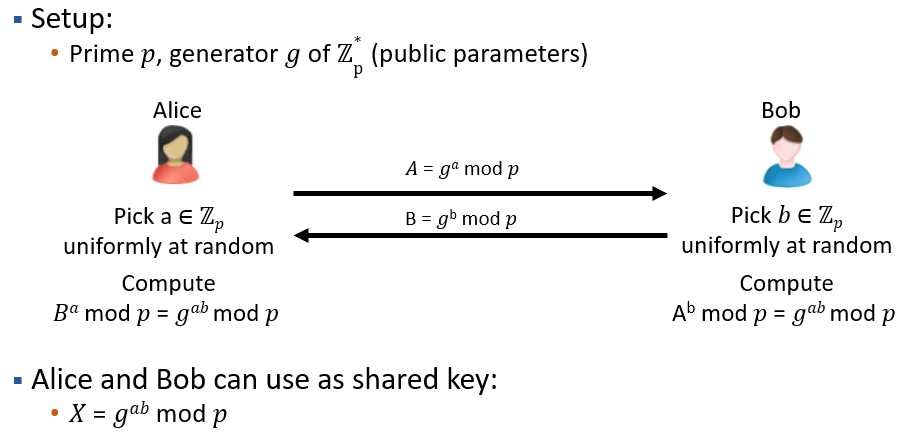
\includegraphics[width=0.7\columnwidth]{images/dh-protocol.jpg}
		\caption{Diffie Hellman Protocol} \label{fig:dh-protocol}
	\end{figure}
	\begin{enumerate}
		\item Design an extension of the Diffie-Hellman protocol to allow secure key exchange between the three parties.\\
		
		\begin{answer}
			
			The below method can be used to extend the DH protocol to share a common key between three parties. The method is graphically represented in the Figure \ref{fig:dh-protocol-extension} as well. The answer was adopted from \url{https://crypto.stackexchange.com/a/1027}
			
			\begin{figure}[H]
				\centering
				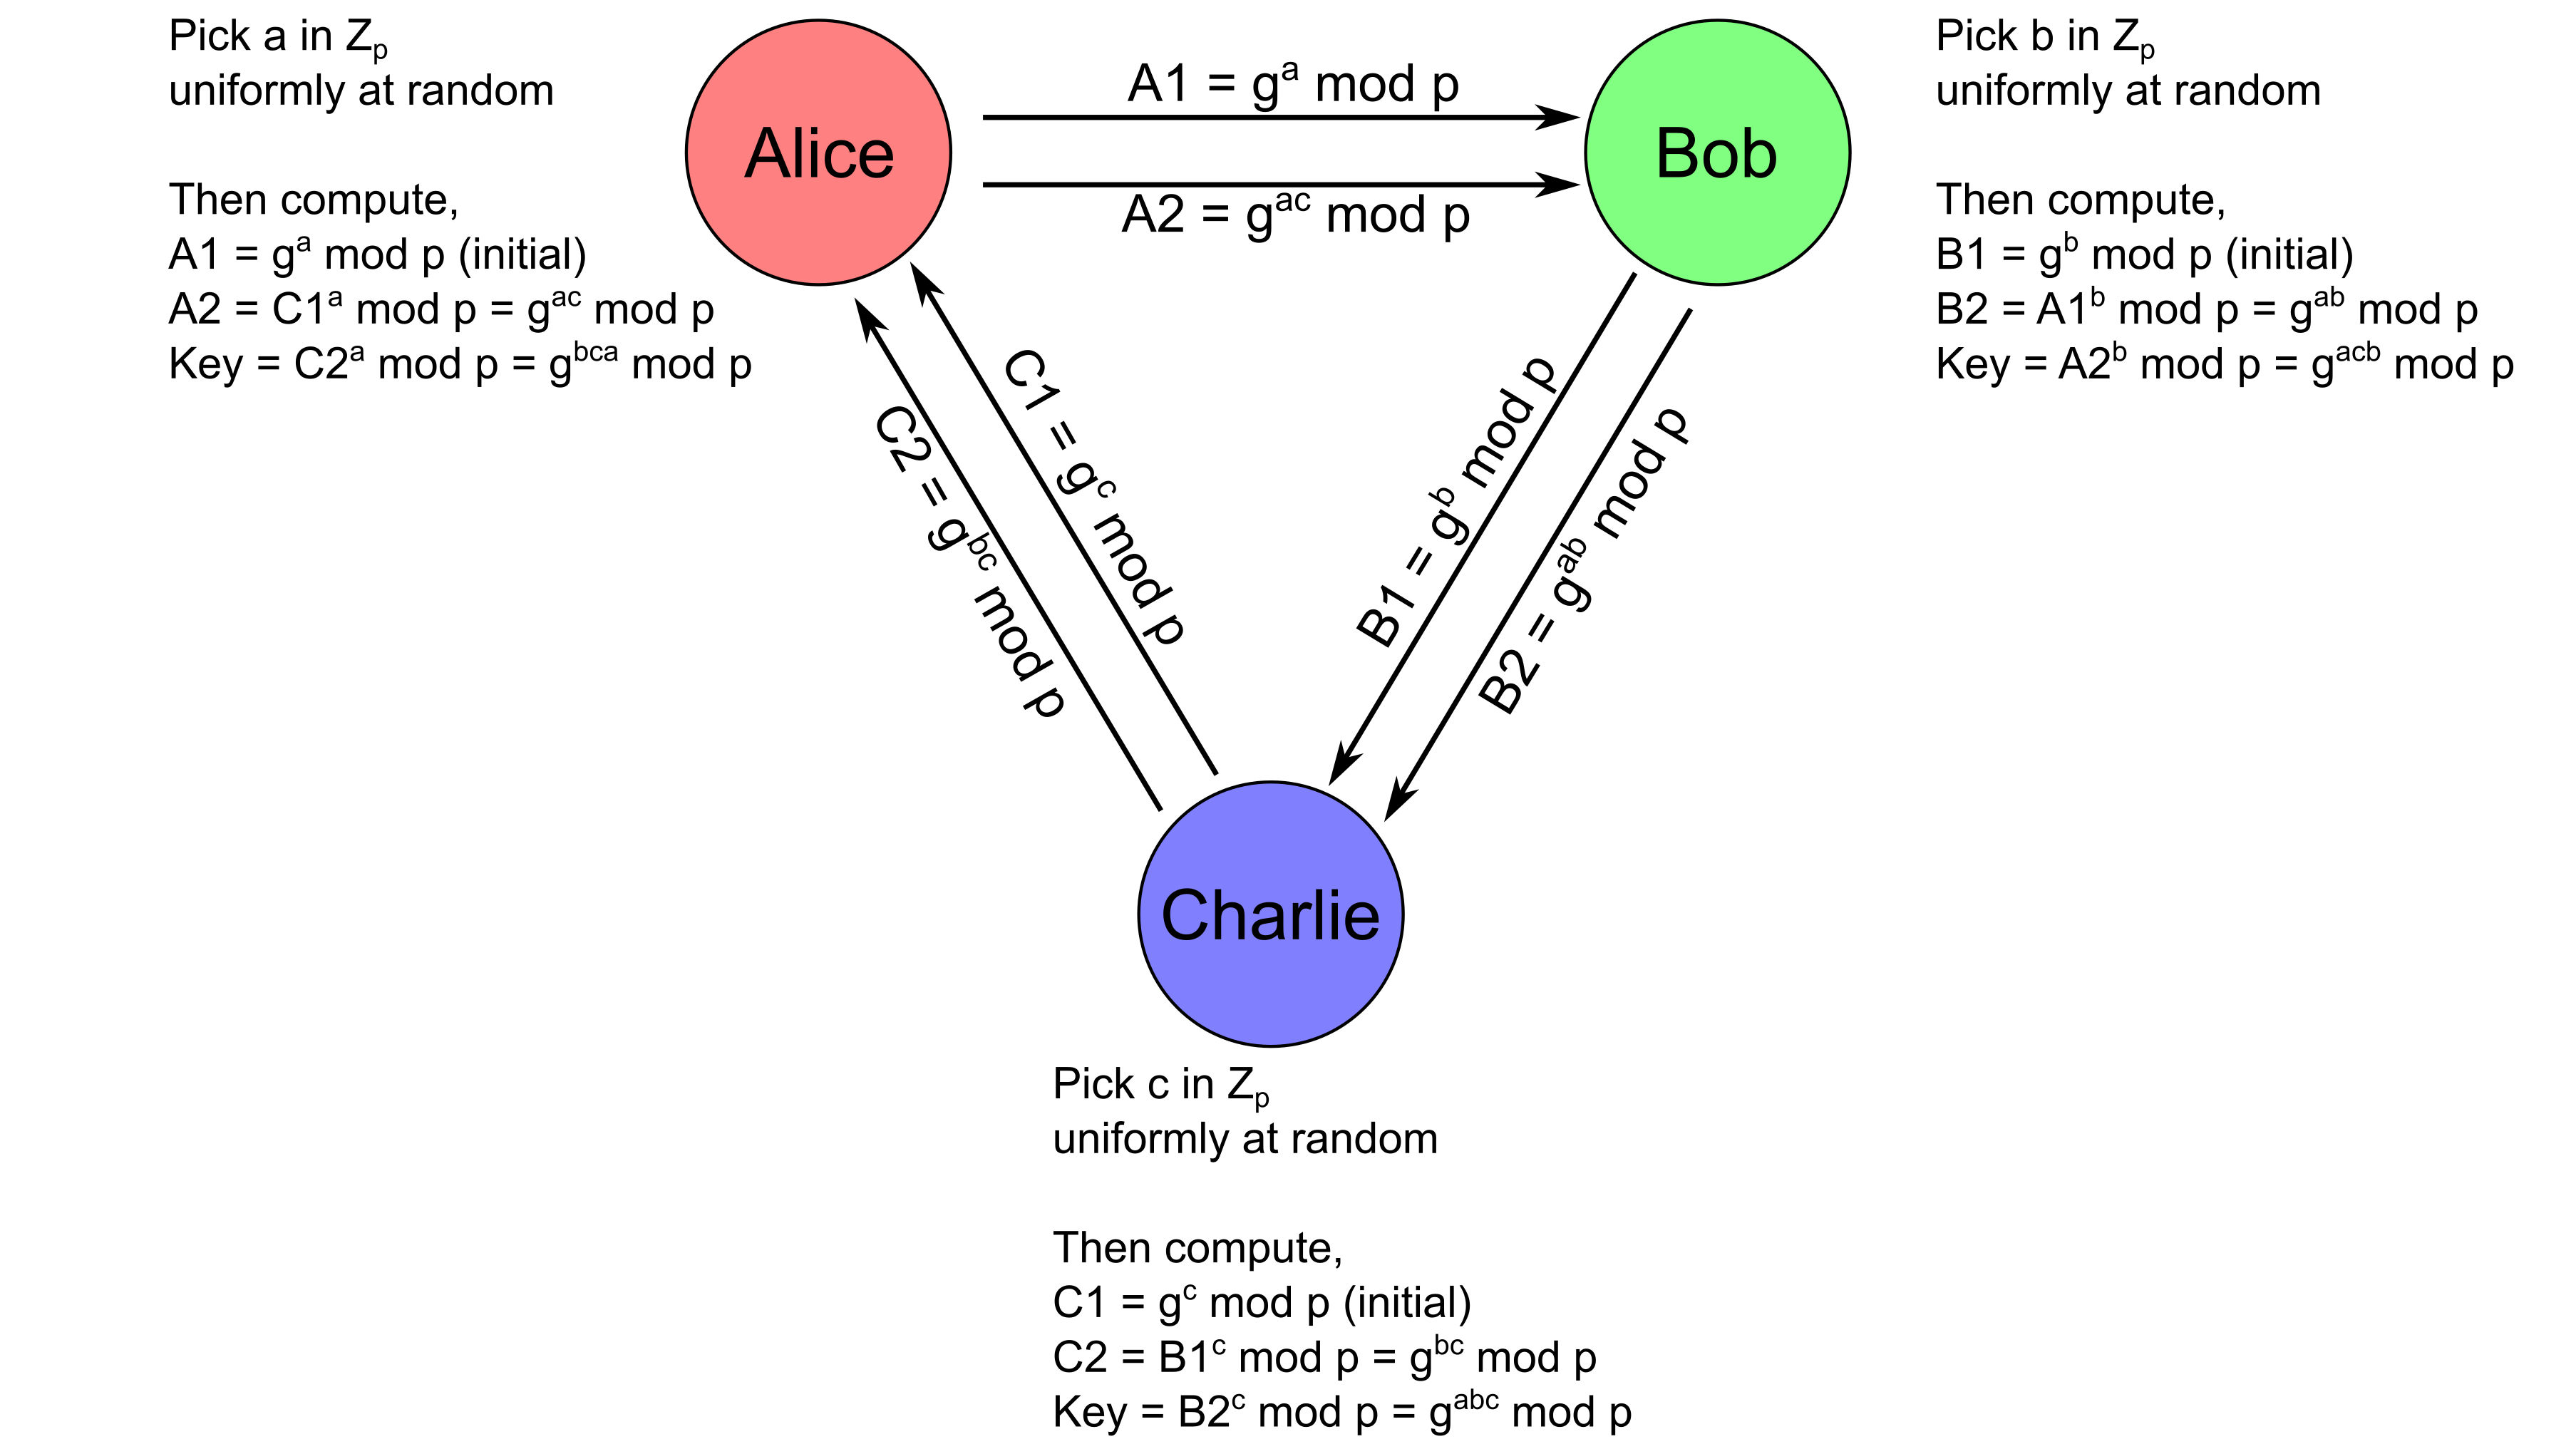
\includegraphics[width=0.7\columnwidth]{images/3-parties-1-key.png}
				\caption{Extended Diffie-Hellman Protocol for three parties to share a common key} \label{fig:dh-protocol-extension}
			\end{figure}
		
		\begin{enumerate}
			\item Alice, Bob and Charlie each picks a random number from the chosen multiplicative group ($\mathbb{Z}_p$). Let those numbers be a, b and c respectively, and Alice, Bob and Charlie are in a loop.
			
			\item The method repeats for two rounds. In the first round each party computes $g^i ~mod~ p$ for the selected $i$ and passes to the next person in the loop.
		\end{enumerate}
		
		\end{answer}
		\item Alice, Bob, and Charlie are planning to use $(p, g) = (23, 9)$ to agree on a key for a Caesar cipher. Assume that the Caesar cipher is right shifting the number of letters equal to the key to produce the ciphertext (e.g., if the key is 5 and the plaintext letter is U, it will be replaced by Z in the ciphertext). Assuming 4, 7, and 13 to be secret exponents of Alice, Bob, and Charlie respectively, find the common key that they need to use in Caesar's cipher.
		\begin{answer}
			%% TODO: Add answer here
			% Sample answer
			Your answer here
		\end{answer}
		\item Derive the encrypted message for the message ``Hello" using the above encryption key.  Show all the major steps in deriving the answer.
		\begin{answer}
			%% TODO: Add answer here
			% Sample answer
			Your answer here
		\end{answer}
	\end{enumerate}
	
	\newpage 
	
	\subsection*{Problem 2 - Symmetric Encryption - Security Analysis}
	For this part of the exercise you are required to install \href{https://www.cryptool.org/en/ct1/}{CrypTool}. CrypTool is a software tool that comes with several encryption techniques.  
	
	\subsubsection*{Instructions}
	\begin{enumerate}
		\item Create a text file named \textbf{``sampletext.txt"} in your computer. Add the text ``EN4720: This is a sample text file for encryption." to the text file and save it.
		\item Open the \textbf{``sampletext.txt"} file with CrypTool software.
		\item Encrypt your message with RC2 encryption following \textbf{Encrypt/Decrypt \textgreater Symmetric (modern) \textgreater RC2}. Choose key size of 8 bits and add some random hexadecimal key to encrypt your text file. (Add screenshots)
		\item Run brute force analysis of the encrypted message by following \textbf{Analysis \textgreater Symmetric Encryption (modern) \textgreater RC2}. (Add screenshots)
		\item Repeat steps 3,4 for the key sizes 16, 24, 64, and 128 bits.
		\item Answer the questions given below.
	\end{enumerate}
	
	\subsubsection*{Questions}
	
	\begin{enumerate}
		\item Add screenshots requested in Step \#3.
		\begin{answer}
			%% TODO: Add answer here
			% Sample answer
			Your answer here
		\end{answer}
		
		\item Add screenshots requested in Step \#4.
		\begin{answer}
			%% TODO: Add answer here
			% Sample answer
			Your answer here
		\end{answer}
		\item Complete Table~\ref{tab:time-taken-to-bruteforce}.
		\begin{table}[h!]
			\caption{Time taken to brute force} \label{tab:time-taken-to-bruteforce}
			\begin{tabularx}{\columnwidth}{|p{4cm}|X|X|}
				\hline
				\textbf{Key length (bits)} & \textbf{Time to brute force} & \textbf{Maximum number of keys} \\
				\hline
				8 & & \\\hline
				
				\hline
				16 & & \\\hline
				
				\hline
				24 & & \\ \hline
				
				\hline
				64 & & \\ \hline
				
				\hline
				128 & & \\ \hline
				
			\end{tabularx}
		\end{table}
		\item What is the impact of key length on time to decrypt a message using brute force?
		\begin{answer}
			%% TODO: Add answer here
			% Sample answer
			Your answer here
		\end{answer}
		\item What could be done to diminish the amount of time required to perform the attack?
		\begin{answer}
			%% TODO: Add answer here
			% Sample answer
			Your answer here
		\end{answer}
		
	\end{enumerate}
	
	\subsection*{Problem 3 - Public Key Encryption}
	
	You are given that $n=65$ and $\phi(n)=48$ for a certain RSA scheme.
	\begin{enumerate}
		\item Calculate the private key $d$ assuming the public key $e=7$.
		\item Show all major steps of encryption and decryption using textbook RSA for the message given below. Specifically, derive the ciphertext and show that the plaintext can be recovered at the receiver after decrypting.\\
		$m=$ last digit of your index number (e.g., if the index number is 180234N, $m=4$). If the last digital is 0 (zero) or 1 (one), use $m=5$. 
		\item Find the candidates for the primes $p,q$ that were used to generate this RSA scheme.
		\item Suppose that $c$ is the ciphertext that you find above for the message $m$. Show how an attacker can recover the plaintext message $m$ from the ciphertext $c$ assuming that he can request a decryption of a single ciphertext $c' \neq c$. 
	\end{enumerate}
	
	\subsection*{Problem 4 - Hash Functions}
	
	{For this part of the exercise you are required to install \href{https://www.kali.org/get-kali/#kali-platforms}{Kali Linux}. Kali Linux comes preinstalled with several hashing utilities. These include \textbf{md5sum}, \textbf{sha1sum},
		\textbf{sha256sum}, and \textbf{sha512sum}. Follow the given instructions to complete the problem.}
	
	\subsubsection*{Instructions}
	\begin{enumerate}
		\item Create a new directory and a new text file ``\textbf{originalhashfile}'' in the directory using \textbf{nano originalhashfile} command. Add the text ``EN4720: Some text here'' in the created file and save the file using the hotkey \textbf{CTRL+X} followed by \textbf{Y} and \textbf{Enter}.
		
		\item Run the \textit{ls} command in the directory to show the file (add screenshot) and run the \textit{cat} command to show the contents of the created file (add screenshot).
		
		\item calculate the hash digest of the \textbf{originalhashfile} using these hash algorithms: MD5, SHA1, SHA256, SHA512 (add screenshots). Add your observations in Table~\ref{tab:hash-digest-originalhashfile}. You can use the following commands to get the results.
		\begin{itemize}
			\item md5sum \textless \textit{hashfile\_name}\textgreater
			\item sha1sum \textless \textit{hashfile\_name}\textgreater
			\item sha256sum \textless \textit{hashfile\_name}\textgreater
			\item sha512sum \textless \textit{hashfile\_name}\textgreater
		\end{itemize}
		
		\item Change the contents of the \textbf{originalhashfile} by adding your index at the end of the line (``EN4720: Some text here \textless\textit{index\_no}\textgreater'') and save it as ``\textbf{modifiedhashfile}'' in the same directory.
		
		\item Run the \textit{ls} command in the directory to show the files (add screenshot) and run the \textit{cat} command to show the contents of the modified file (add screenshot).
		
		\item Calculate the hash digest of the \textbf{modifiedhashfile} using these hash algorithms: MD5, SHA1, SHA256, SHA512 (add screenshots). Add your observations in Table~\ref{tab:hash-digest-modifiedhashfile}.
		
		\item Answer the questions given below.
		
	\end{enumerate}
	\newpage
	\subsubsection*{Questions}
	\begin{enumerate}
		
		\item Add screenshots requested in Step \#2.
		
		\begin{answer}
			%% TODO: Add answer here
			% Sample answer
			Your answer here
		\end{answer}
		
		% \begin{figure}[h!]
			% \centering
			% \includegraphics[scale=1]{images/ex2_hashing_sol1.png}
			% \label{fig:ex2_hashing_sol1}
			% \end{figure}
		
		
		\item Complete Table~\ref{tab:hash-digest-originalhashfile}. Add screenshots requested in Step \#3 below the table.
		
		% \begin{table}[h!]
			%     \caption{Hash digests of the original file
				%     } \label{tab:hash-digest-originalhashfile}
			%     \begin{tabularx}{\columnwidth}{|p{4cm}|X|}
				%         \hline
				%         \textbf{Hash Algorithm} & \textbf{Hash of the Original File} \\
				%         \hline
				%         MD5 & caf4d10c96b7b646e24ae72f366b4c7d \\\hline
				
				%         \hline
				%         SHA1 & e64870421f78773bf65437f515fd384170ce8839 \\\hline
				
				%         \hline
				%         SHA256 & cc544b593a0faa91f34774289a66b7400d1ce3fa36cfaec64a958228c5ead764 \\ \hline
				
				%         \hline
				%         SHA512 & cc7aebdfdf19a2f9882deb0ff1fc01a5be9f25cb2b916bd179b4ec88436113c5dc246\\&18487bed98fcc3d11574bafabde3a5c785eed6bccef496a7817d132d73a \\ \hline
				
				%     \end{tabularx}
			% \end{table}
		
		\begin{table}[h!]
			\caption{Hash digests of the original file
			} \label{tab:hash-digest-originalhashfile}
			\begin{tabularx}{\columnwidth}{|p{4cm}|X|}
				\hline
				\textbf{Hash Algorithm} & \textbf{Hash of the Original File} \\
				\hline
				MD5 &  \\\hline
				
				\hline
				SHA1 &  \\\hline
				
				\hline
				SHA256 &  \\ \hline
				
				\hline
				SHA512 &  \\ \hline
				
			\end{tabularx}
		\end{table}
		
		% \begin{figure}[h!]
			% \centering
			% \includegraphics[scale=1]{images/ex2_hashing_sol2.png}
			% \label{fig:ex2_hashing_sol2}
			% \end{figure}
		
		\item Among the hash algorithms used, which one is the most cryptographically secure? Justify your answer.
		
		\begin{answer}
			%% TODO: Add answer here
			Your answer here
		\end{answer}
		
		\item Why is MD5 not considered as a reliable hashing algorithm?
		
		\begin{answer}
			%% TODO: Add answer here
			Your answer here
		\end{answer}
		
		\item Which of the algorithms fall under the category of SHA-2?
		\begin{answer}
			%% TODO: Add answer here
			Your answer here
		\end{answer}
		
		\item Add screenshots requested in Step \#5.
		
		\begin{answer}
			%% TODO: Add answer here
			% Sample answer
			Your answer here
		\end{answer}
		
		% \begin{figure}[h!]
			% \centering
			% \includegraphics[scale=1]{images/ex2_hashing_sol3.png}
			% \label{fig:ex2_hashing_sol3}
			% \end{figure}
		
		\item Complete Table~\ref{tab:hash-digest-modifiedhashfile}. Add screenshots requested in Step \#6 below the table.
		
		% \begin{table}[h]
			%     \caption{Hash digests of the modified file
				%     } \label{tab:hash-digest-modifiedhashfile}
			%     \begin{tabularx}{\columnwidth}{|p{4cm}|X|}
				%         \hline
				%         \textbf{Hash Algorithm} & \textbf{Hash of the Modified File} \\
				%         \hline
				%         MD5 & 658fb63dcd71f730284c6d924e55baa5\\ \hline
				
				%         \hline
				%         SHA1 & 1c4416490482fafef63f9afb3c8709d76efde1f1\\ \hline
				
				%         \hline
				%         SHA256 & 2ee4b6655994db95f3d0e47f0d7ab43c51cf3bab2363c75a1a92fcc052545ddc \\ \hline
				
				%         \hline
				%         SHA512 & a6da55e69664a3bac0d96daed5f16fec55cb15b956688a2baa88ee5d22a8b59f347\\&470fcd858d8831da0ce5513745f108830ef9baf51104bef492b6d17aae522\\ \hline
				
				%     \end{tabularx}
			% \end{table}
		
		\begin{table}[h]
			\caption{Hash digests of the modified file
			} \label{tab:hash-digest-modifiedhashfile}
			\begin{tabularx}{\columnwidth}{|p{4cm}|X|}
				\hline
				\textbf{Hash Algorithm} & \textbf{Hash of the Modified File} \\
				\hline
				MD5 & \\ \hline
				
				\hline
				SHA1 & \\ \hline
				
				\hline
				SHA256 &  \\ \hline
				
				\hline
				SHA512 & \\ \hline
				
			\end{tabularx}
		\end{table}
		
		% \begin{figure}[h!]
			% \centering
			% \includegraphics[scale=1]{images/ex2_hashing_sol4.png}
			% \label{fig:ex2_hashing_sol4}
			% \end{figure}
		
		\item Comparing the output from one algorithm in Table~\ref{tab:hash-digest-originalhashfile} and Table~\ref{tab:hash-digest-modifiedhashfile}, is there a difference between the hash digests? If yes, why?
		
		\begin{answer}
			%% TODO: Add answer here
			Your answer here
		\end{answer}
		
		% \item Explore ``\href{https://www.slavasoft.com/hashcalc/}{HashCalc}'', ``\href{http://md5deep.sourceforge.net/}{md5deep}'' and ``\href{http://md5deep.sourceforge.net/}{hashdeep}'' tools and summarize their capabilities in three/four sentences each.
		
		% \begin{answer}
			% %% TODO: Add answer here
			% HashCalc: Your answer here
			
			% md5deep: Your answer here
			
			% hashdeep: Your answer here
			
			% \end{answer}
		
	\end{enumerate}
	% \bibliographystyle{plain} % We choose the &quot;plain&quot; reference style
	% \bibliography{refs} % Entries are in the &quot;refs.bib&quot; file</code></pre>
\end{document}
